\section{Design \& Konzept}
\label{sec:design-und-konzept}
In diesem Kapitel ...

\subsection{Grundlegende Designentscheidungen}
Bevor auf Entscheidungen eingegangen wird ...

\subsubsection{Android als Plattform}
Das Framework richtet sich ausschließlich an Entwickler die Applikationen für die Plattform Android entwickeln. Es ist damit nicht kompatibel zu iOS, dem Web oder Serverseitigen Anwendungen. Die Spezialisierung lässt es jedoch zu, besser auf mögliche Eigenheiten der Plattform einzugehen. Ein weiterer Grund für diese Entscheidung stellt die Tatsache dar, dass MVI seinen Anfang in der Entwickelung von Webseiten fand und es sich im Fall Android um einen Nachzügler handelt.

\subsubsection{Framework}
Warum Framwork? Besonderheiten...
\subsection{Übersicht der Komponenten im Klassendiagramm}
\begin{sidewaysfigure}
		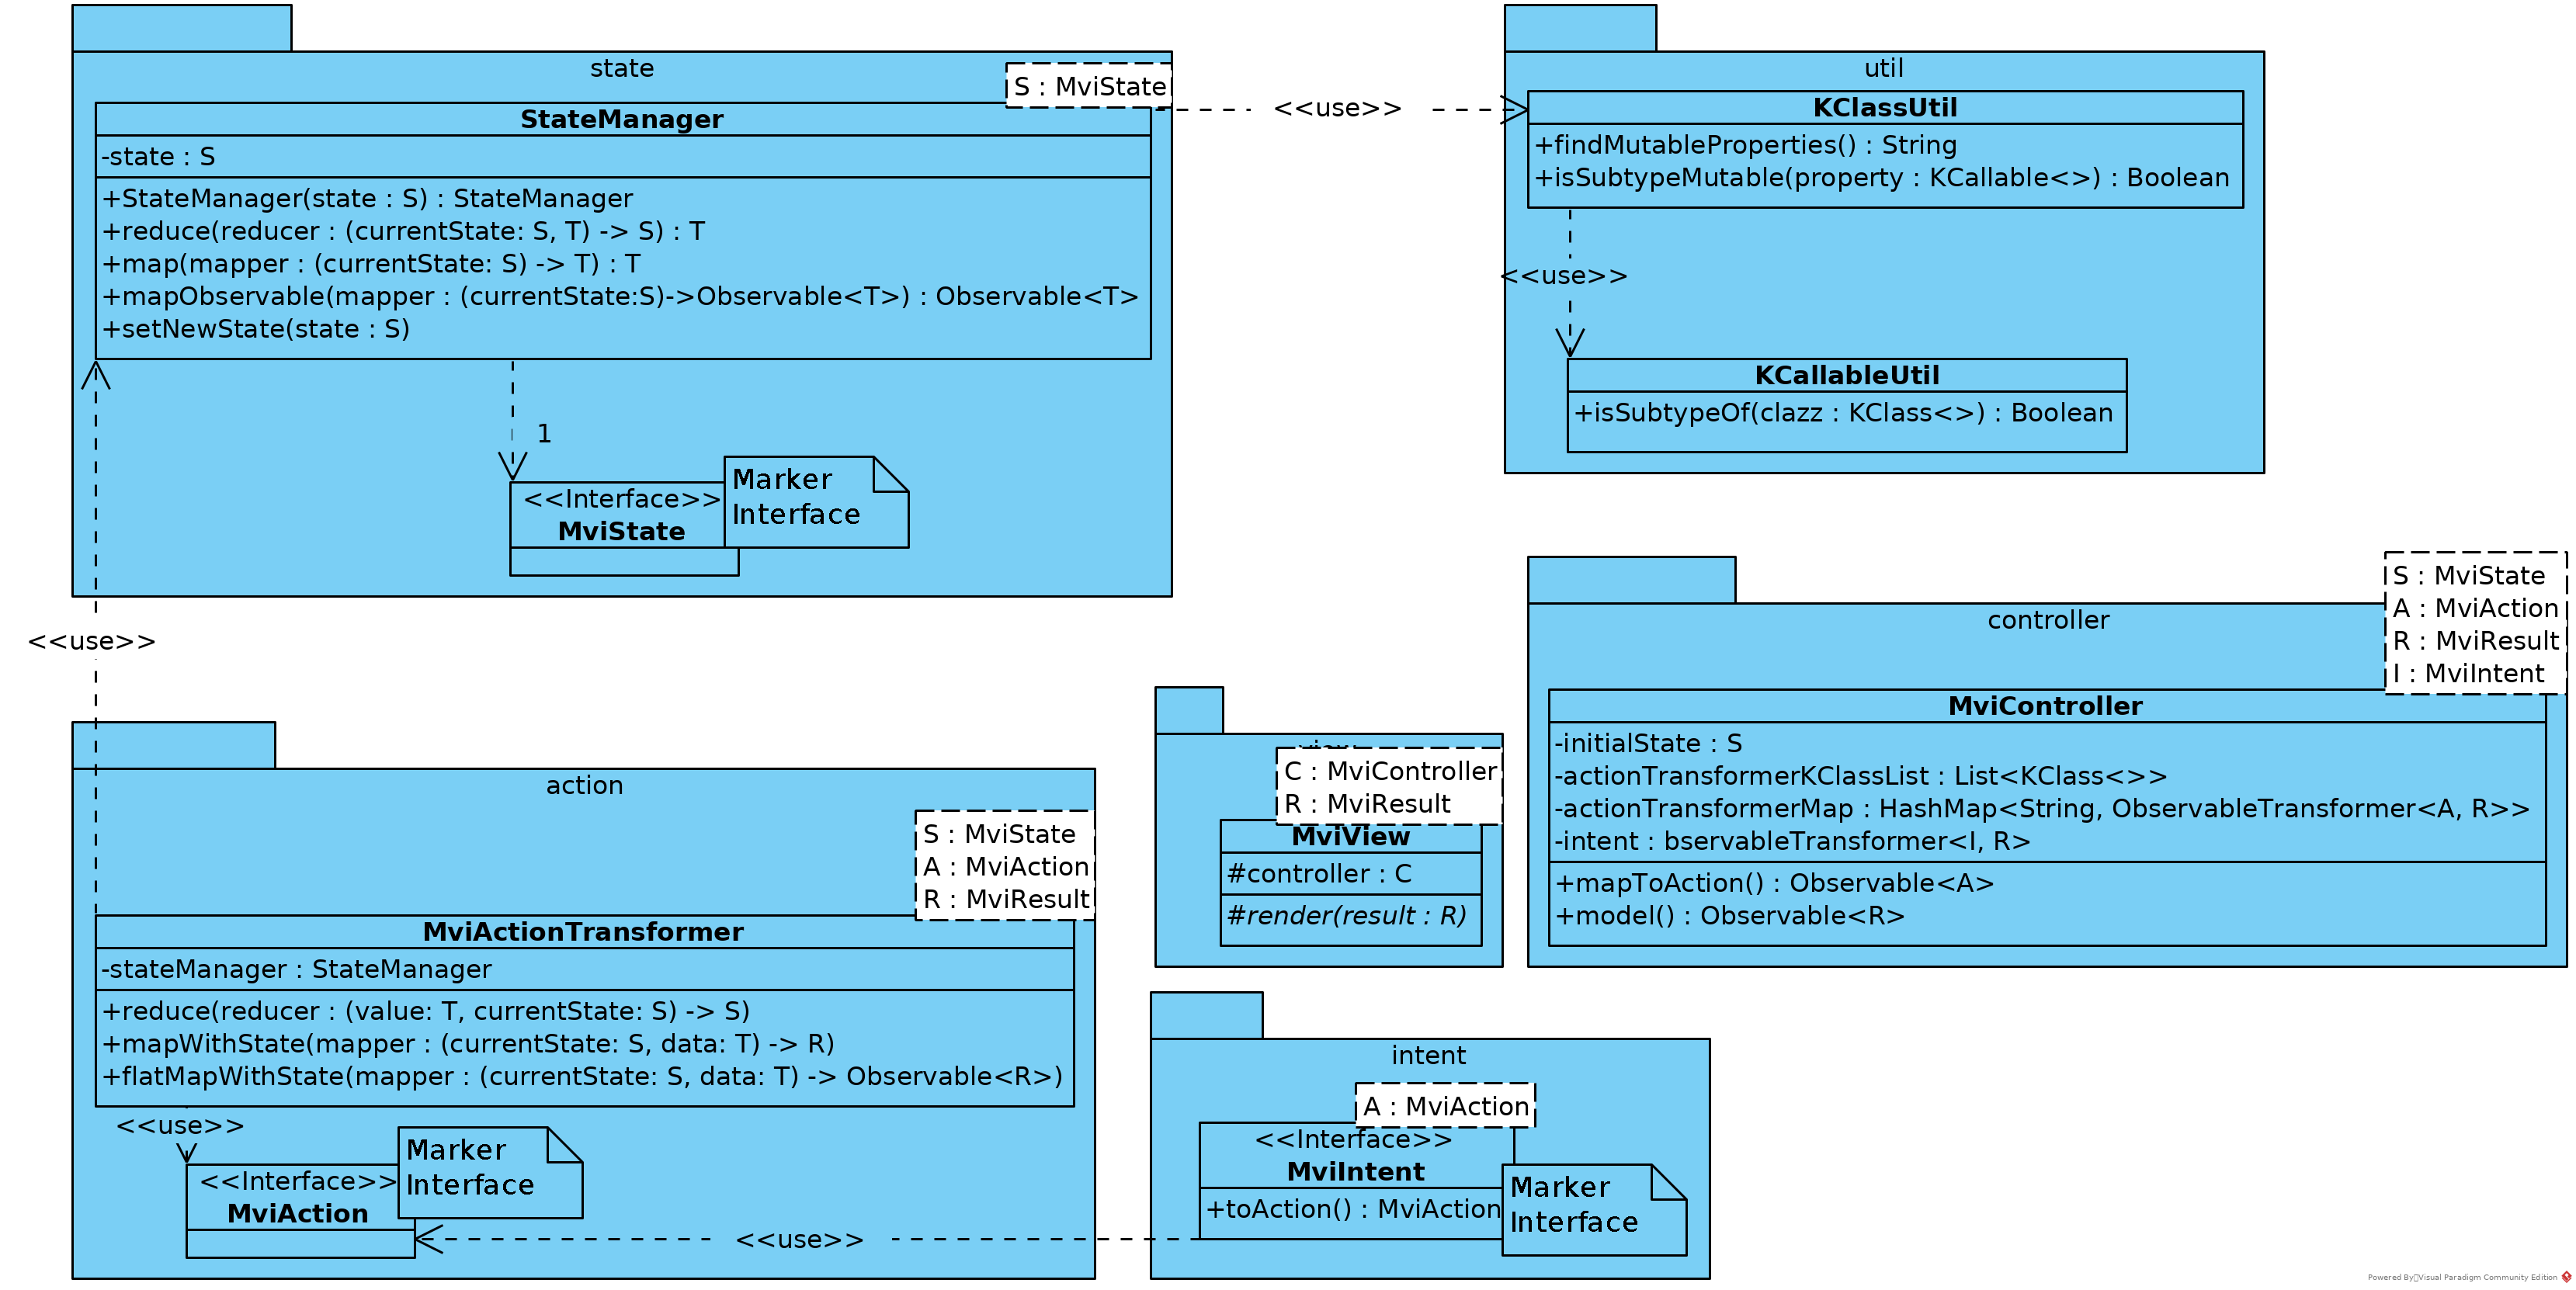
\includegraphics[width=\textwidth]{./images/framework-class-diagram}
		\caption{Komponenten im Klassendiagramm}
\end{sidewaysfigure}
\clearpage
\subsection{Zustand (State) und seine Verwaltung}
In den Ausführungen von MVI wird der Zustand als eine Anhäufung von Werten betrachtet. Es bildet den Kern von MVI und muss im Normalfall vom Entwickler selbst verwaltet werden. Unter anderem muss garantiert sein, dass ein Zugriff und eine Modifikation des Zustands nur an einer Stelle erfolgen kann. Im Rahmen des Framworks wird eine Komponente genutzt, die diese Aufgaben für den Entwickler übernimmt und den Zustand 'managed': Der 'StateManager'.
\\\\
Dieser erwartet den initialen Zustand, der vom Entwickler an das Framework übergeben wird. Der Zustand wird dabei als generischer Parameter definiert und muss dem Interface 'MviState' entsprechen. Nachdem der Zustand überreicht wurde, wird geprüft, inwieweit dieser der Anforderung der Unveränderlichkeit entspricht. Sollte diese nicht gegeben sein, so wird eine Fehlermeldung ausgegeben und der Prozess gestoppt.
\\\\
Ist dies erfolgreich, so wartet der 'StateManager' mit Funktionalität auf, welche es ermöglicht einen neuen Zustand zu hinterlegen, sowie mit ihm sicher zu arbeiten. Ein neue Setzung des Wertes wird dabei durch die Kombinationen der Funktionen 'reduce' und 'setNewState' erreicht. 
\\\\
Erstere erwartet eine Funktion als Parameter, 'reducer', welche wiederum den derzeitigen Zustand übergeben bekommt. Diese wird aufgerufen und produziert einen neuen Zustand, der durch 'setNewState' als aktueller Zustand gesetzt wird. Dies geschieht allerdings nur unter der Prämisse, dass sich mindestens ein Wert innerhalb der Datenstruktur verändert hat.
\\
Als Zusatz stellt 'setNewState' sicher, dass es auch bei gleichzeitigen Zugriffen von mehreren 'Threads' zu keiner sogenannten unbeabsichtigten Wettlaufsituation (Race Condition) und damit schwer auffindbaren Problemen kommt.
\\\\
Die Methode 'map' nimmt genau wie 'reduce' eine Funktionen entgegen, welche den aktuellen Zustand erhält. In dieser kann der Entwickler auf die Attribute des Zustands zurückgreifen, jedoch keine neuen bestimmen.
\\\\
Diese Komponente ist nicht direkt für den Nutzer zugänglich und wir ausschließlich intern im Framework genutzt. Es verhindert, dass der Zustand an einer beliebigen und nicht vorgesehenen Stelle verändert werden kann.

\subsection{Intent, Action und Result}
Die im Titel genannten Komponenten dienen der Übermittlung und Beschreibung von Informationen innerhalb des 'Kreislaufs' vom MVI. Diese müssen vom Entwickler selbst gestellt werden, erhalten dabei jedoch Vorgaben vom Framework.
\\\\
So muss zu jedem Intent eine Action existieren. Hierfür wartet das Framework mit dem Interface 'MviIntent' auf, das genanntes erzwingt und die Erfüllung dieser Anforderung sicherstellt. Realisiert wird dies durch die Funktion 'mapToAction', die der Entwickler später implementieren muss und eine 'Action' zurück gibt.  
\\\\
Ähnlich wie auf einen Intent eine Action erfolgt, zieht eine Action ein Result nach sich. Auch das gibt das Framework durch ein Interface namens 'MviAction' vor und muss vom Entwickler angewandt werden. Das Result findet seine Anwendung später in der View und wird ebenfalls mit einem Interface versehen.
\\
\\
Sämtliche der hier aufgeführten Strukturen sollten mit ihrem Namen die vorgesehene Intention signalisieren. Zusätzlich müssen sie in der Lage sein weitere Nutzdaten (Payload) aufzunehmen, die mit ihnen in Zusammenhang stehen und für den weiteren Verlauft Essential sind.

\subsection{Reaktiver unidirektionaler Datenfluss}
Für die Konzeptionierung der nächsten Komponenten gilt vorher zu klären, wie der geforderte reaktive unidirektionale Datenfluss in das Framework integriert werden soll. Dabei müssen Daten synchron oder asynchron verarbeitet und die Option zur Nebenläufigkeit (Concurrency) geboten werden. Zu diesem Zweck bedarf es einem Tool, welches das bereits aufgeführte 'Observer' und 'Iterator' Pattern nutzt. In diesem Zusammenhang taucht oft das Objekt 'Observable' auf, das genau diese Anforderungen erfüllt.  

\subsection{Transformer und die Business-Logik}
Ein elementaren Bestandsteil einer Anwendung macht die Businesslogik aus. Sie ist im Falle von MVI allein verantwortlich für das Abändern des Zustands und sollte strikt von anderen Komponenten getrennt sein.
Hierfür stellt das Framework den 'ActionTransformer zu Verfügung.
\\\\
Wie der Name vermuten lässt, ist die 'Action' unter anderem ausschlaggebend für die Nutzung der Komponente. Jeder 'Action' wird dabei ein 'ActionTransfomrer' zuteil, welcher über der ersten der zwei generischen Parameter, dem 'A', definiert wird. Dieser Parameter setzt voraus, dass das eingesetzte Objekt vom Interface 'MviAction' nutzen macht. Der zweite generische Parameter 'R' sieht ein Objekt vor, dass dem Interface 'MviResutlt' entstammt. Hier wird das zugehörige Result zur angegebenen Action eingefügt. 
\\\\
Der 'ActionTransformer' ermöglicht die Interaktion mit dem Zustand durch eine Variationen an Funktionen. Dafür benötigt er einen 'StateManager' welcher im bei seiner Erstellung übergeben werden muss. Die Funktionalität kann dabei - ähnlich wie beim 'StateManger' - in zwei Kategorien unterteilt werden:
\begin{enumerate}
	\item Die, in der ein neuer Zustand erzeugt wird und
	\item die, in der ausschließlich auf die Daten zugegriffen wird
\end{enumerate} 
Zu ersten Kategorie gehört lediglich die 'reduce' Methode, welche auf die gleichnamige Methode im 'StateManager' zugreift. 
\\\\
Somit ist im Quellcode klar ersichtlich, inwieweit eine Abänderung der Zustands gewollt ist und wann dieser lediglich mitsamt seiner Daten für den weiteren Verlauf benötigt wird. Hinzu kommt hier auch die automatische Handhabung von Seiteneffekten und asynchroner Funktionalität. Dies garantiert, dass der Zustand keine unabsichtliche Modifikation erfährt und zu jedem Zeitpunkt nur einer auf ihn zugreifen kann.

\subsection{Controller}
Der Controller vereint die bisher beschriebenen Komponenten und 'kontrolliert' bzw. koordiniert anhand dieser den Aufruf der Business-Logik. Er stellt das Bindeglied zwischen der View, einer 'Action' und dem dazugehörigen 'ActionTransormer' dar und sorgt für den Aufruf von ebendiesem. Dafür muss er über die vom Entwickler angedachte Form des Zustands, Intents, Action und Result informiert werden. Überdies erhält der Controller den initialen Zustand und eine Liste von Namen der zugehörigen 'ActionTransformer' vom Entwickler.
\\\\
In der initialen Phase verifiziert er daraufhin, dass alle 'ActionTransformer' von der hinterlegten 'Action' und dem 'Result' abstammen um späteren Konflikten vorzubeugen. Anschließend wird der 'StateMananger' mit dem überlieferten Zustand instanziiert. Im letzten Schritt erzeugt der Controller alle 'ActionTransformer' die jeweils einen 'StateManager' zugewiesen bekommen.
\\\\
Im Controller befindet sich die Intent-Funktionen, welche die von der View generierten 'Intents' entgegennimmt und verarbeitet. Sie dient als Einstiegspunk in den unidirektional Kreislauf. Ebenfalls findet hier die Model-Funtionen ihren Platz, welche allerdings nicht für den Entwickler sichtbar ist und intern automatisch abgewickelt wird. Sie trägt Sorge für den Aufruf des korrekten 'ActionTransformers'. 

\subsection{View}
Die 'View' stellt den obersten Teil des Frameworks dar und gibt an, 

\subsection{Anleitung zur korrekten Nutzung}
Hier wird (Schritt für Schritt) beschrieben wie der Entwickler zu Verfahren hat, um das Framework zu nutzen.